\chapter{Secret appendix}
You are now reading the secret appendix!
A place hosting information classified due reasons such as: high variance, unreliable controls, missing validations, partial knockouts, swapped labels, performed by undergrads, irregular proliferation, high background, bad antibodies, pipetting accidents, wrong volume, low signal etc. etc. etc.



\section{Integrated stress response}

\subsection{Aspartate depletion induced ISR}

Media swapping induces a quick depletion of both Asp and Asn
If Asp is depleted to the point of protein synthesis inhibition no signal might be detected as Asp levels will not recover.
On the other hand if Asn is depleted it can activate ISR while being produced at sufficient amounts to reveal ISR through ATF4.


\begin{figure}
    \centering
    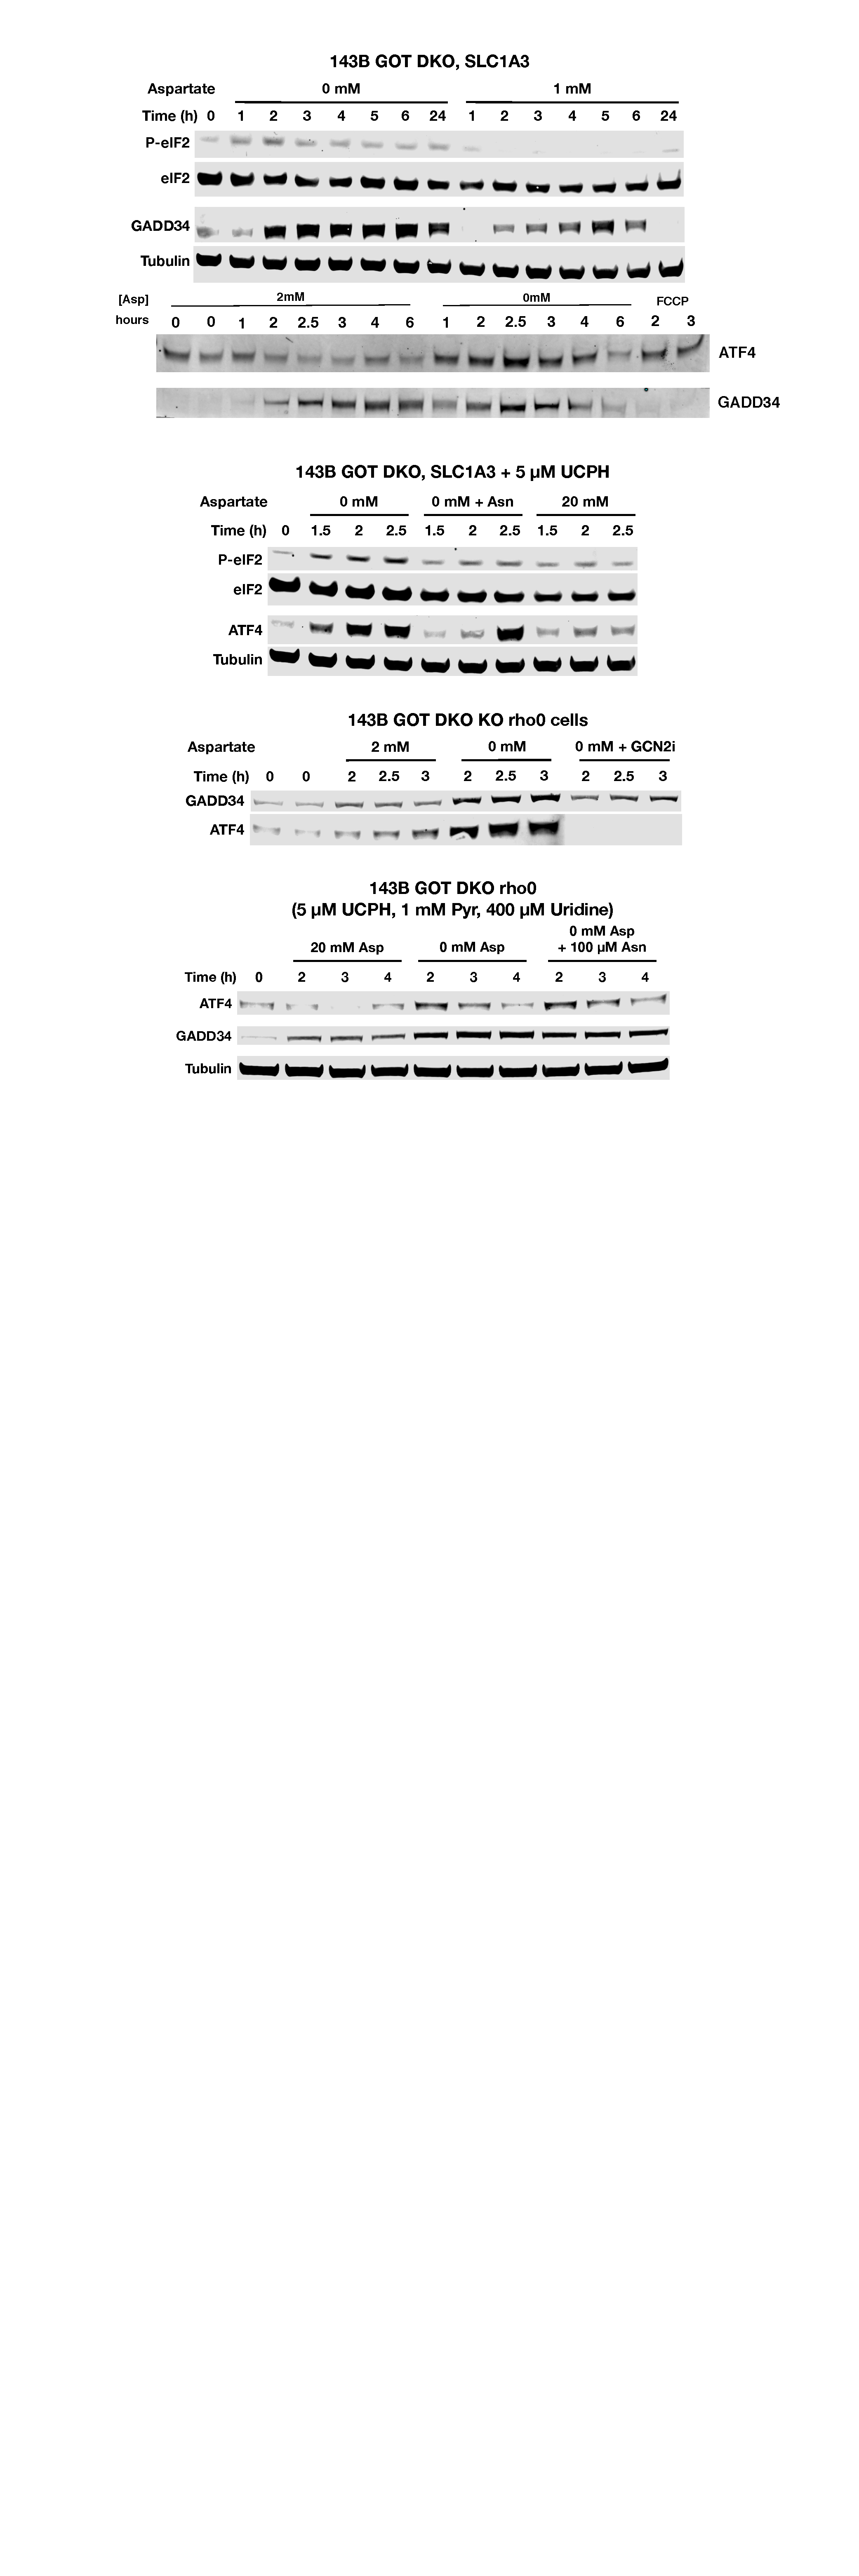
\includegraphics[height=0.85\textheight]{figures/sapp/ISR/143B_DKO_ISR.pdf}
    \caption[Asp depl. induced ISR, 143B]{
    Aspartate depletion in 143B GOT DKO, SLC1A3 cells initiated by media swapping.
    }
    \label{fig:sapp:ISR:143B_DKO_ISR}
\end{figure}

\begin{figure}
    \centering
    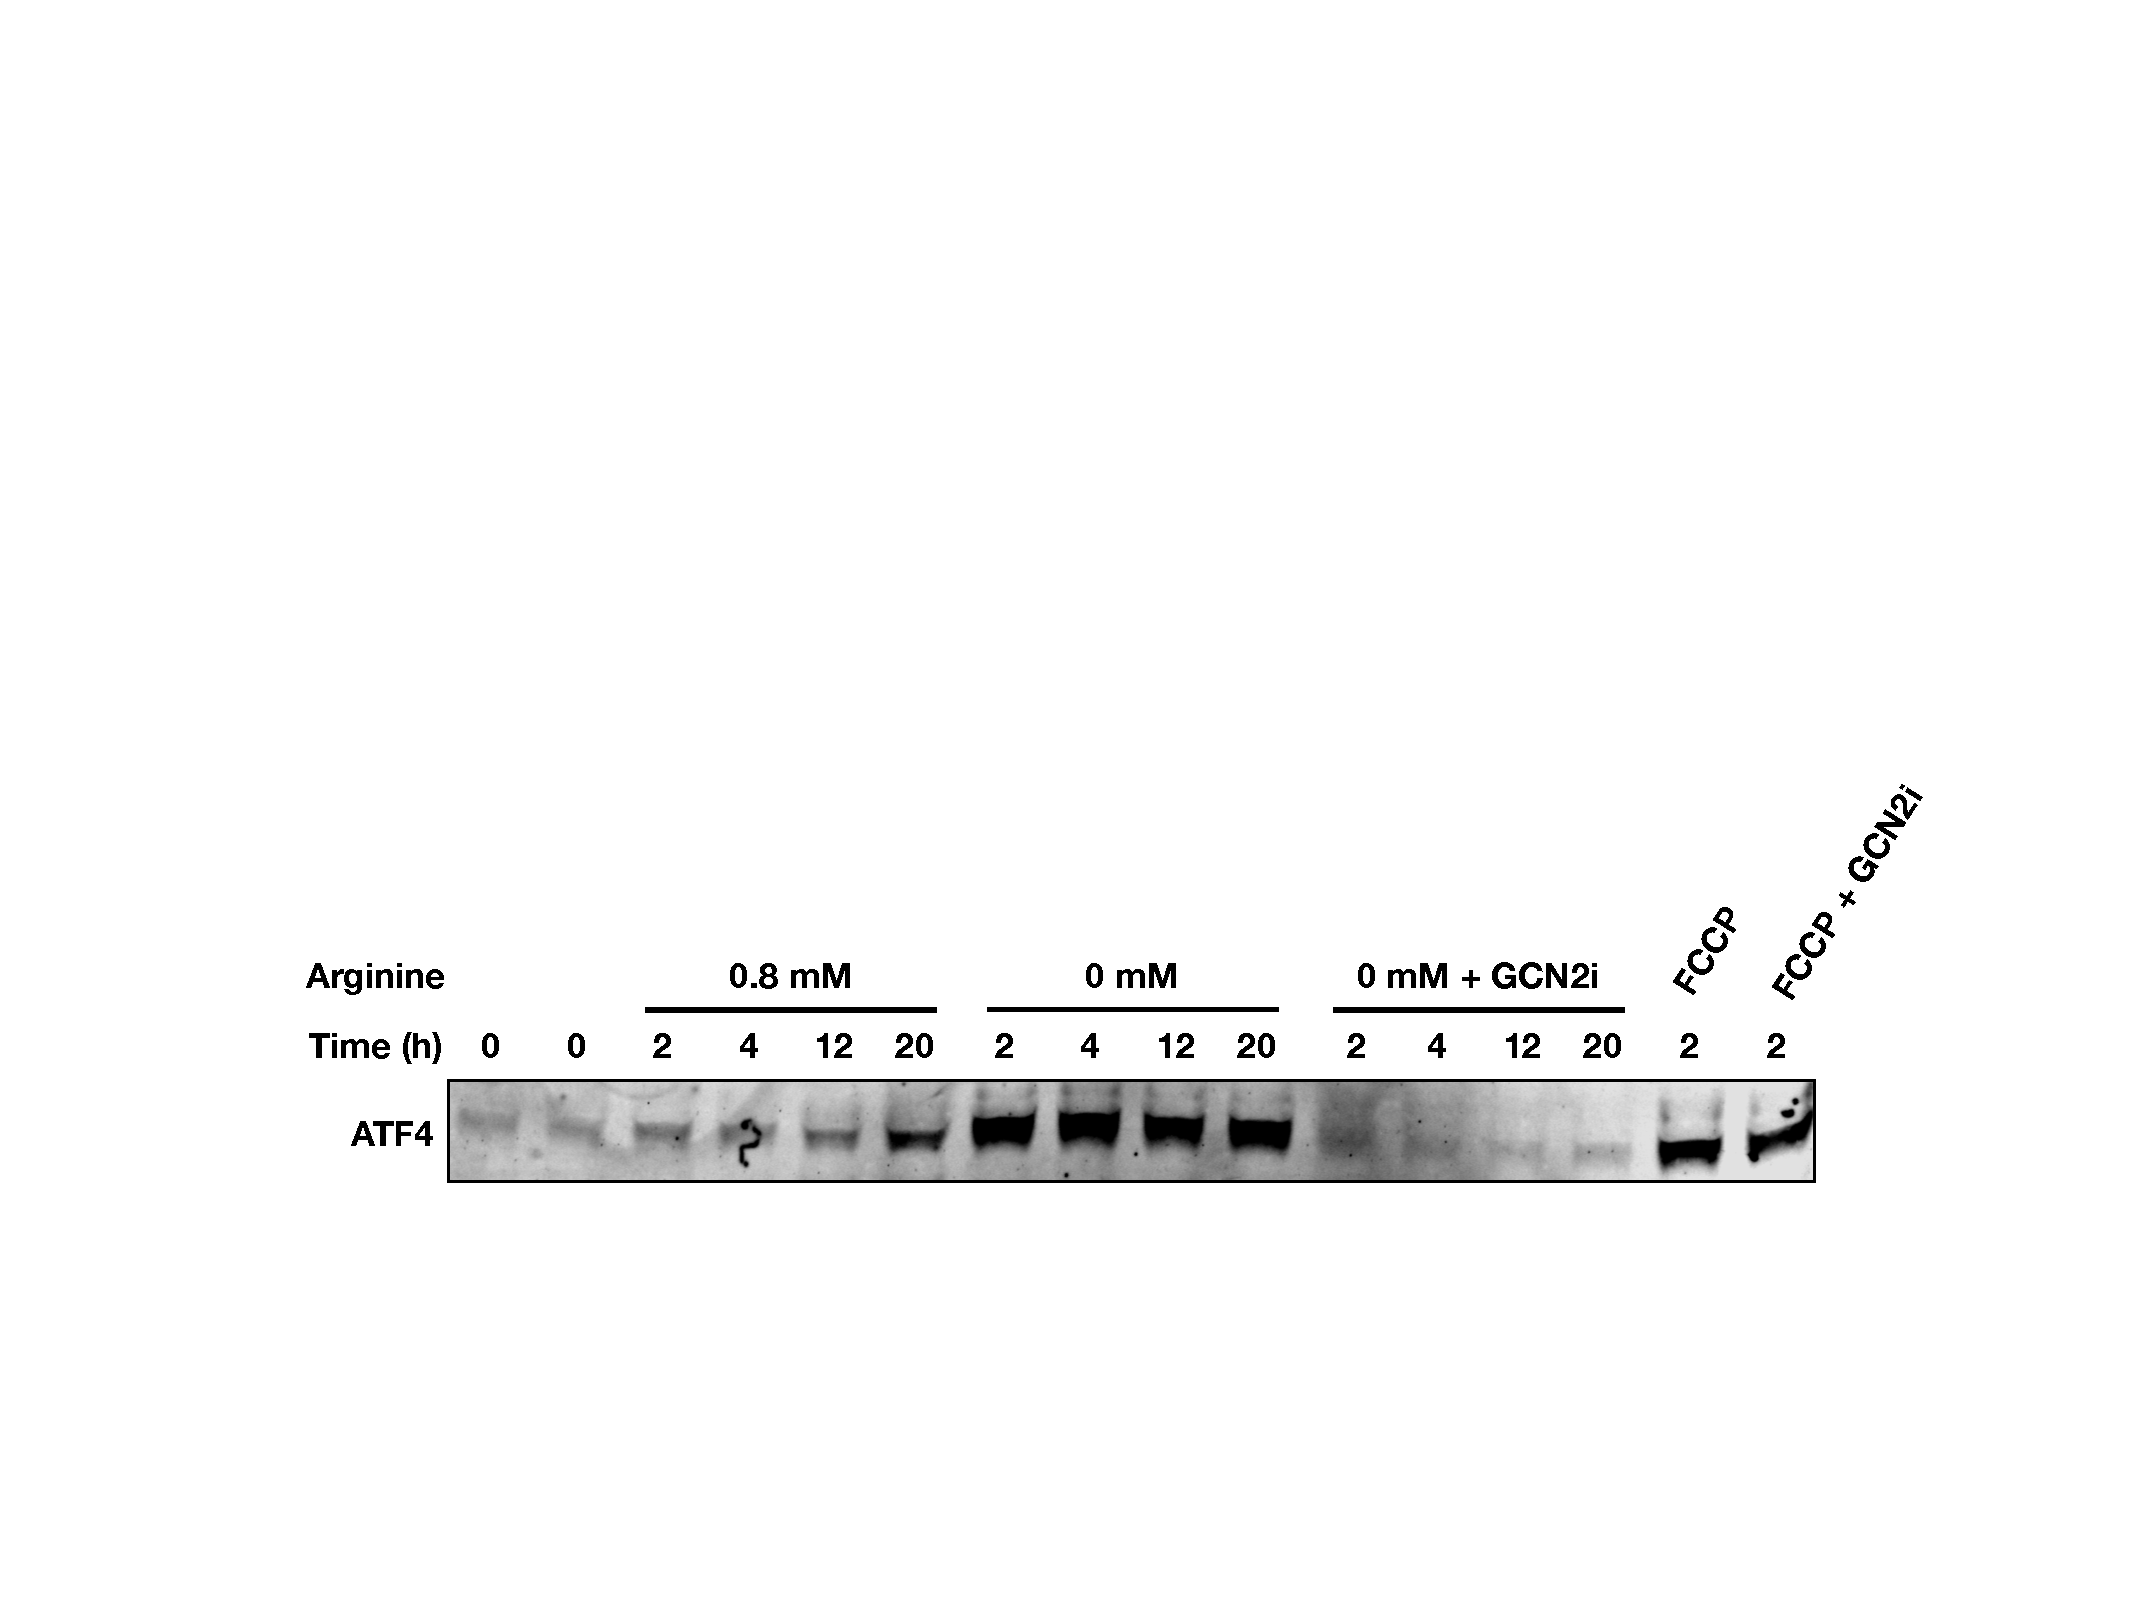
\includegraphics[width=0.60\textwidth]{figures/sapp/ISR/143B_GCN2i_val.pdf}
    \caption[GCN2i validation]{
    Validation of activity and specificity of GCN2i in 143B WT cells.
    }
    \label{fig:sapp:ISR:143B_GCN2i_val}
\end{figure}



\begin{figure}
    \centering
    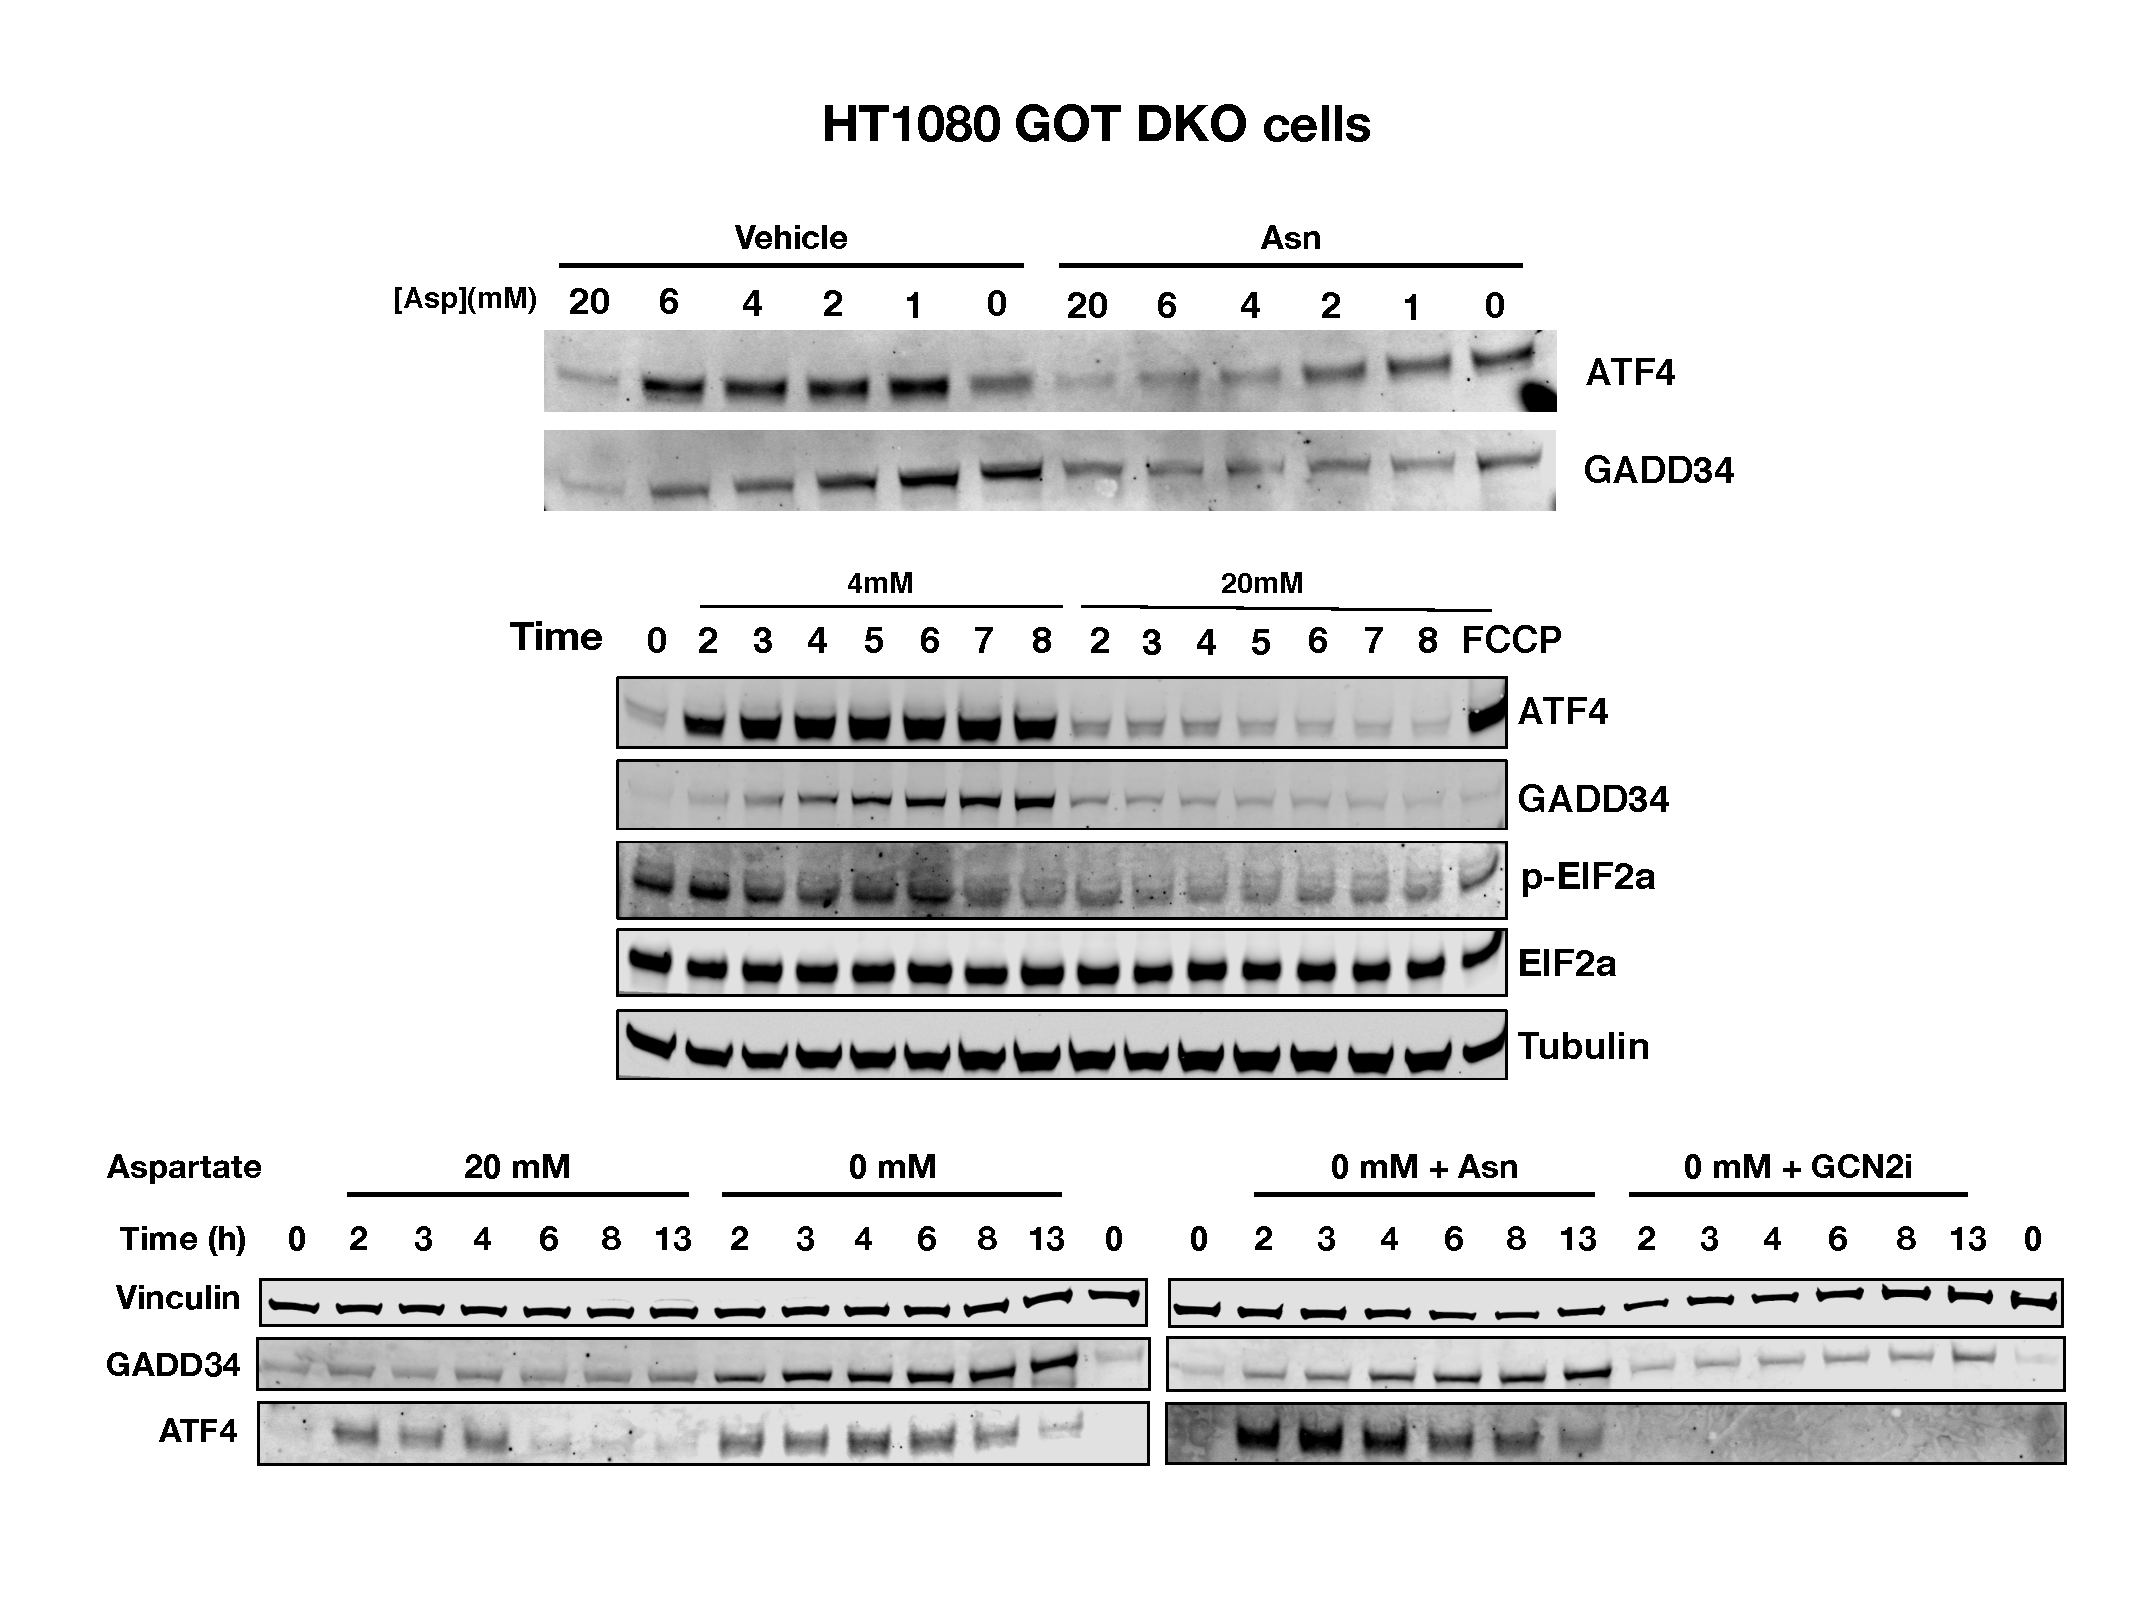
\includegraphics[width=0.99\textwidth]{figures/sapp/ISR/HT1080_DKO_ISR.pdf}
    \caption[Asp depl. induced ISR, HT1080]{
    Aspartate depletion in HT1080 GOT DKO cells initiated by media swapping.
    }
    \label{fig:sapp:ISR:HT1080_DKO_ISR}
\end{figure}

\begin{figure}
    \centering
    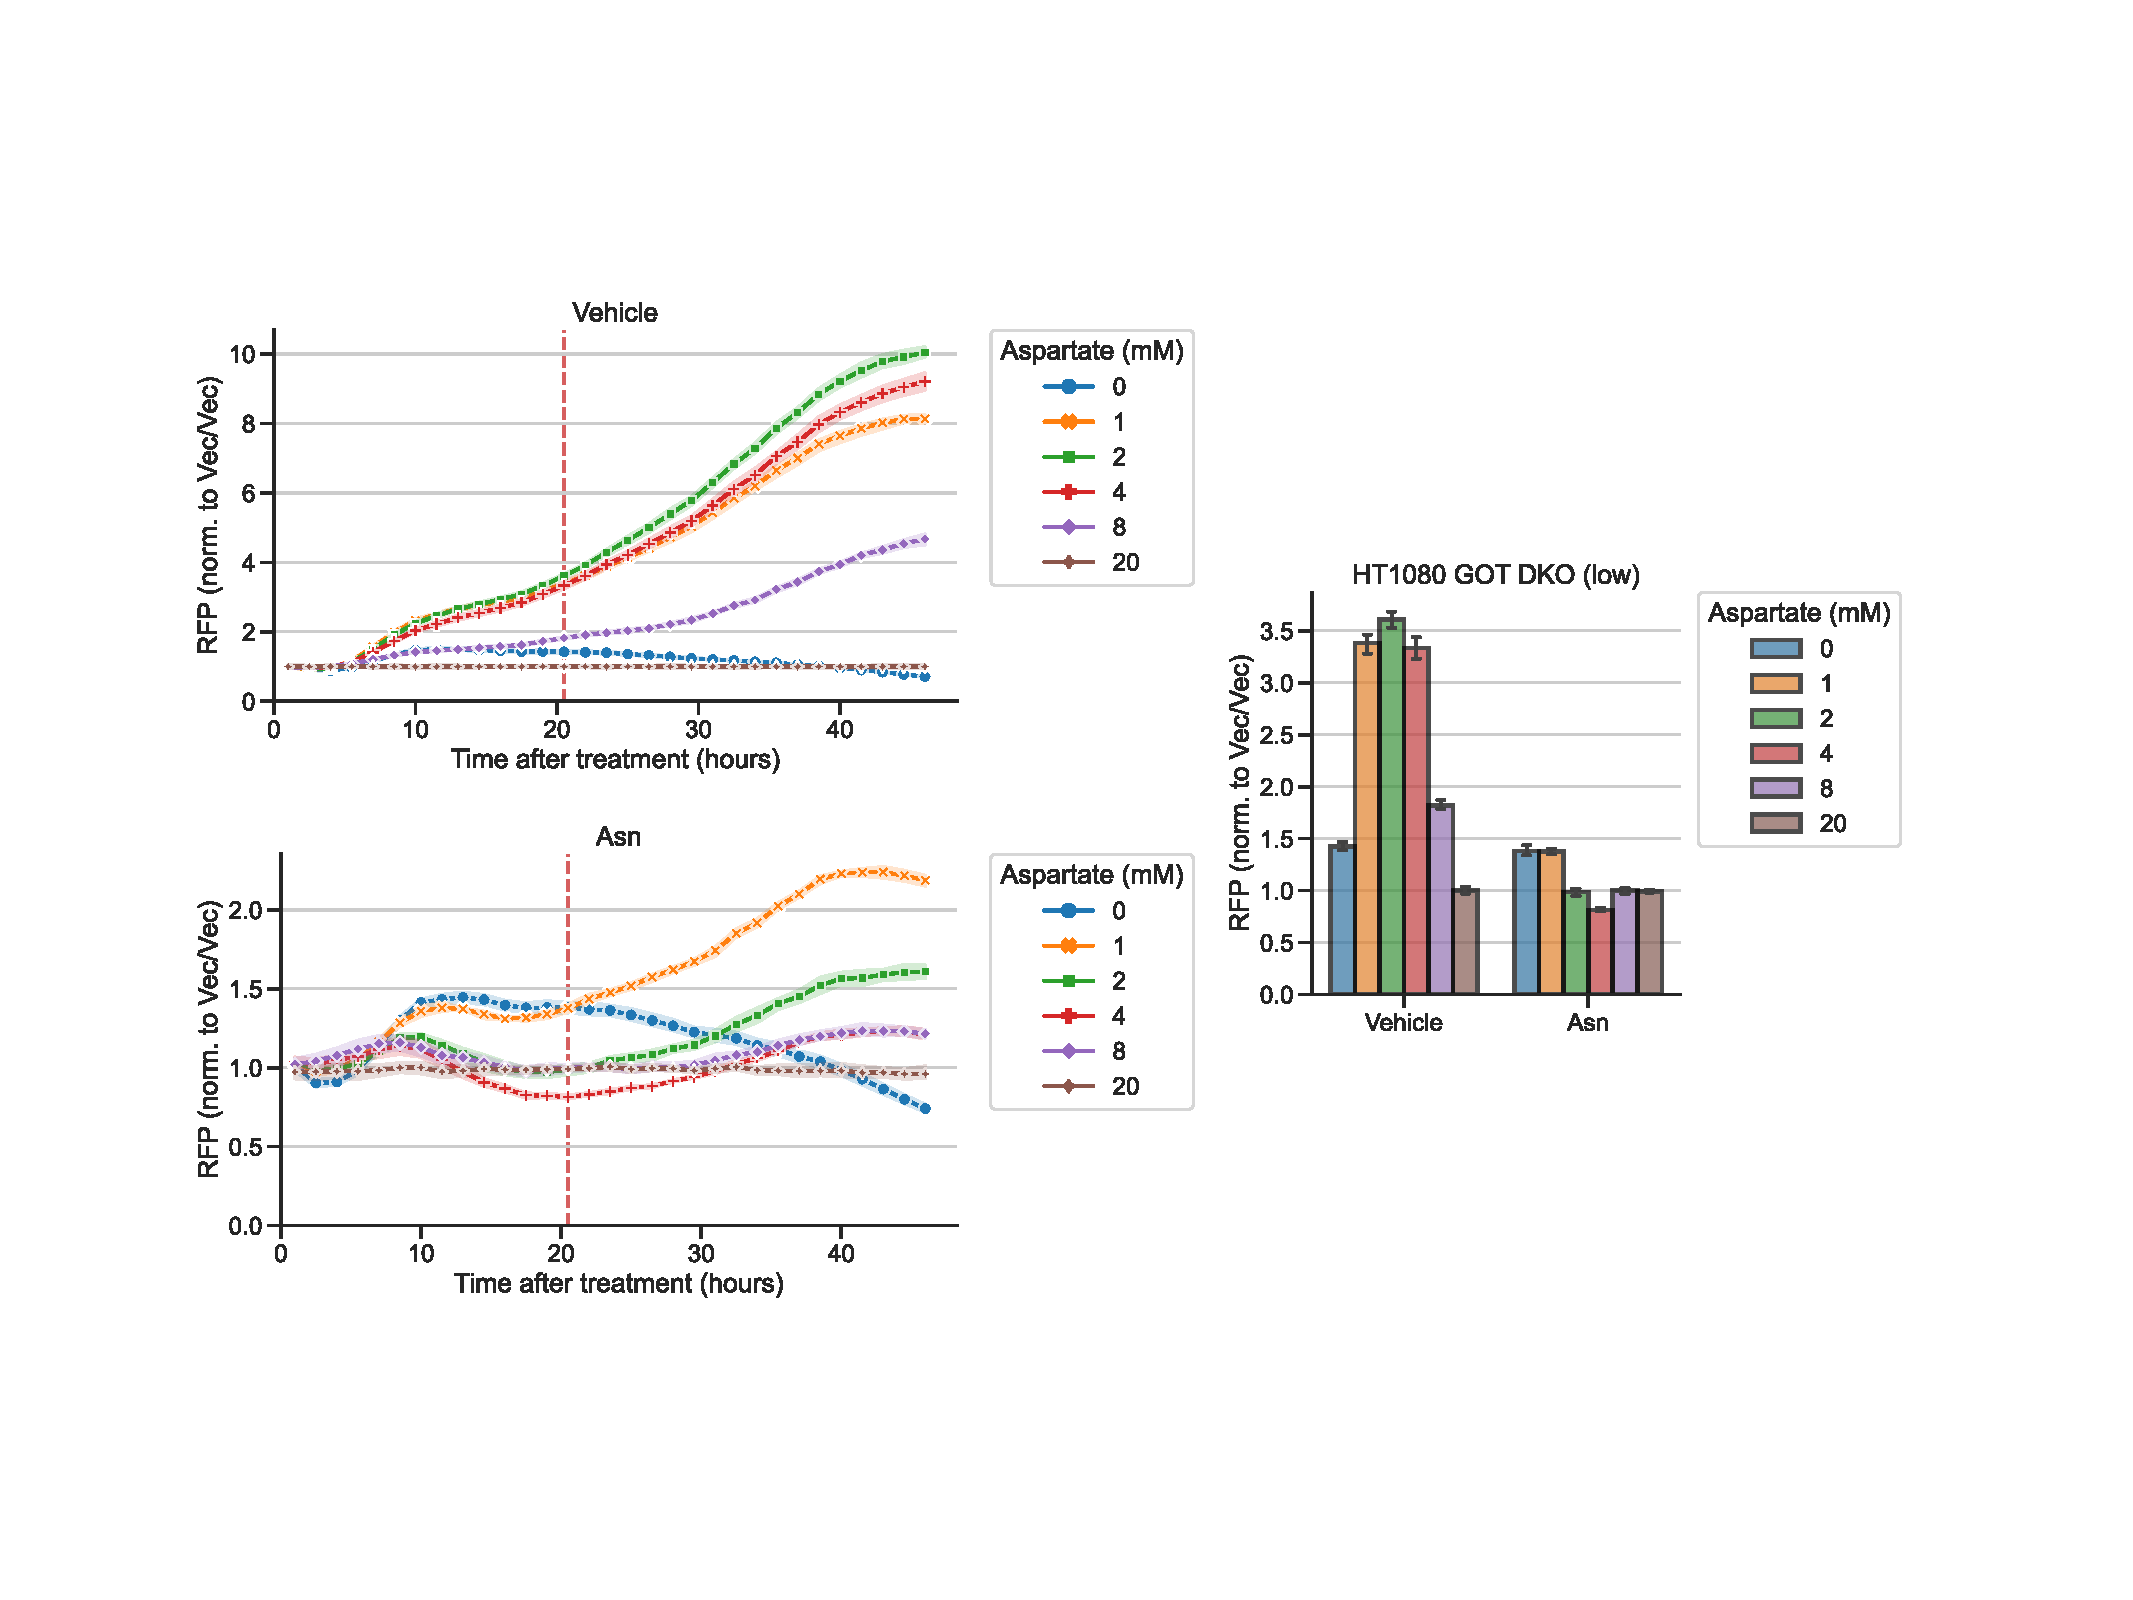
\includegraphics[width=0.98\textwidth]{figures/sapp/ISR/HT1080_DKO_ASPtit_time.pdf}
    \caption[Asp depl. induced ISR, HT1080 ATF4 reporter]{
    ATF4 reporter measurements after aspartate depletion in HT1080 GOT DKO (clone with low reporter at baseline).
    Vec/Vec normalization is normalization to the baseline condition (20 mM Asp, no Asn).
    }
    \label{fig:sapp:ISR:HT1080_DKO_ASPtit_time}
\end{figure}









\subsection{OMA1/HRI relation to rotenone/antimycin induced ISR}
According Fessler et al. and Guo et al. \cite{Fessler2020-zk, Guo2020-ia} OMA1/HRI is required for FCCP induced ISR, as well as rotenone/antimycin induced ISR (suppl. of Guo et al.).

\begin{figure}
     \centering
     \begin{subfigure}[b]{0.49\textwidth}
         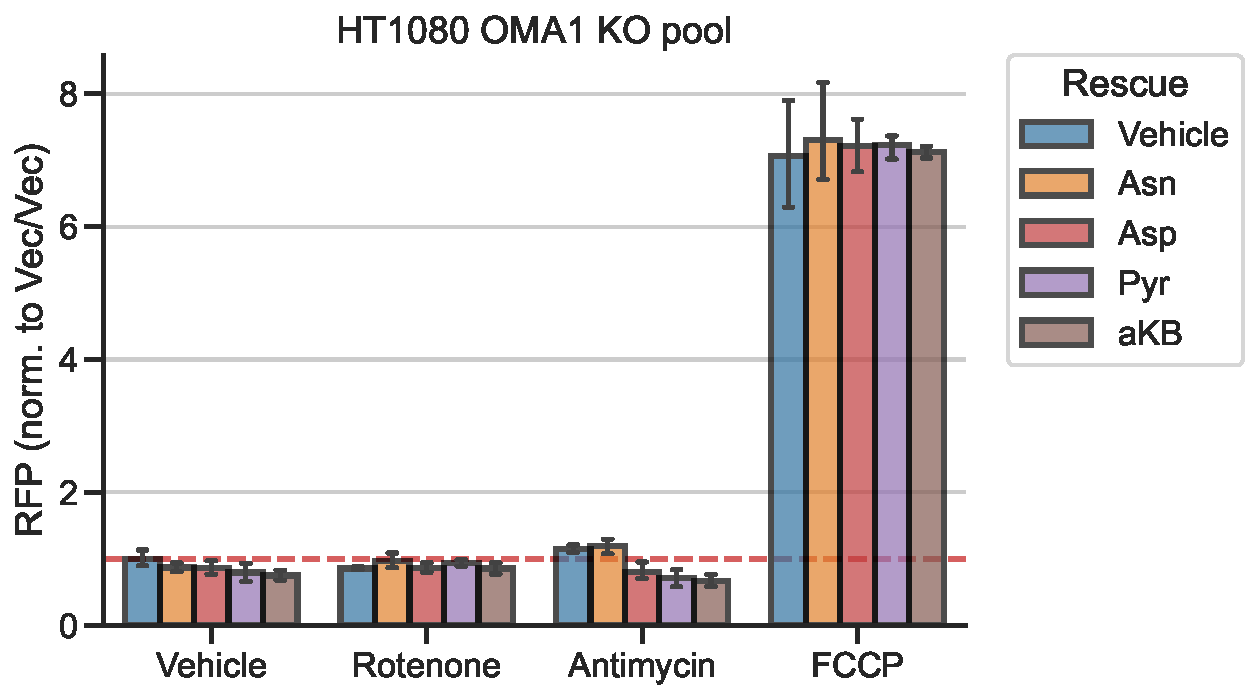
\includegraphics[width=\textwidth]{figures/sapp/ISR/ATF4rep_OMA1pool.pdf}
         \caption{OMA1 KO pool}
         \label{fig:sapp:ISR:ATF4rep_OMA1pool}
     \end{subfigure}
     \hfill
     \begin{subfigure}[b]{0.49\textwidth}
         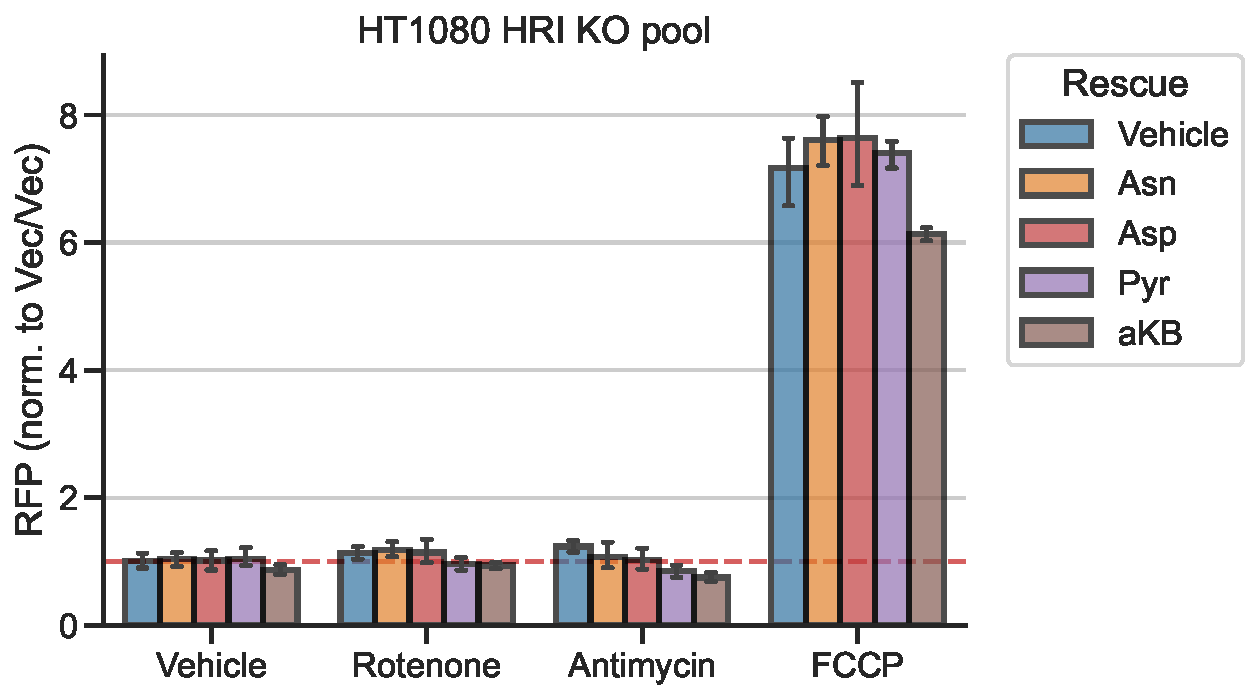
\includegraphics[width=\textwidth]{figures/sapp/ISR/ATF4rep_HRIpool.pdf}
         \caption{HRI KO pool}
         \label{fig:sapp:ISR:ATF4rep_HRIpool}
     \end{subfigure}
     \hfill
        \caption[ATF4 post mito inhib. OMA1/HRI KO, reporter]{
        ATF4 reporter assay measured 21 h after drug treatment with vehicle, rotenone (100 nM) or antimycin (1 µM) spiked-in as 10x.
        In these pooled knockout cells (parental HT1080 ATF reporter low clone) OMA1/HRI KO appears to ablate rotenone/antimycin induced ISR but strangely not FCCP induced ISR.
        }
        \label{fig:sapp:ISR:ATF4rep_OMA1_HRIpool}
\end{figure}

\begin{figure}
    \centering
    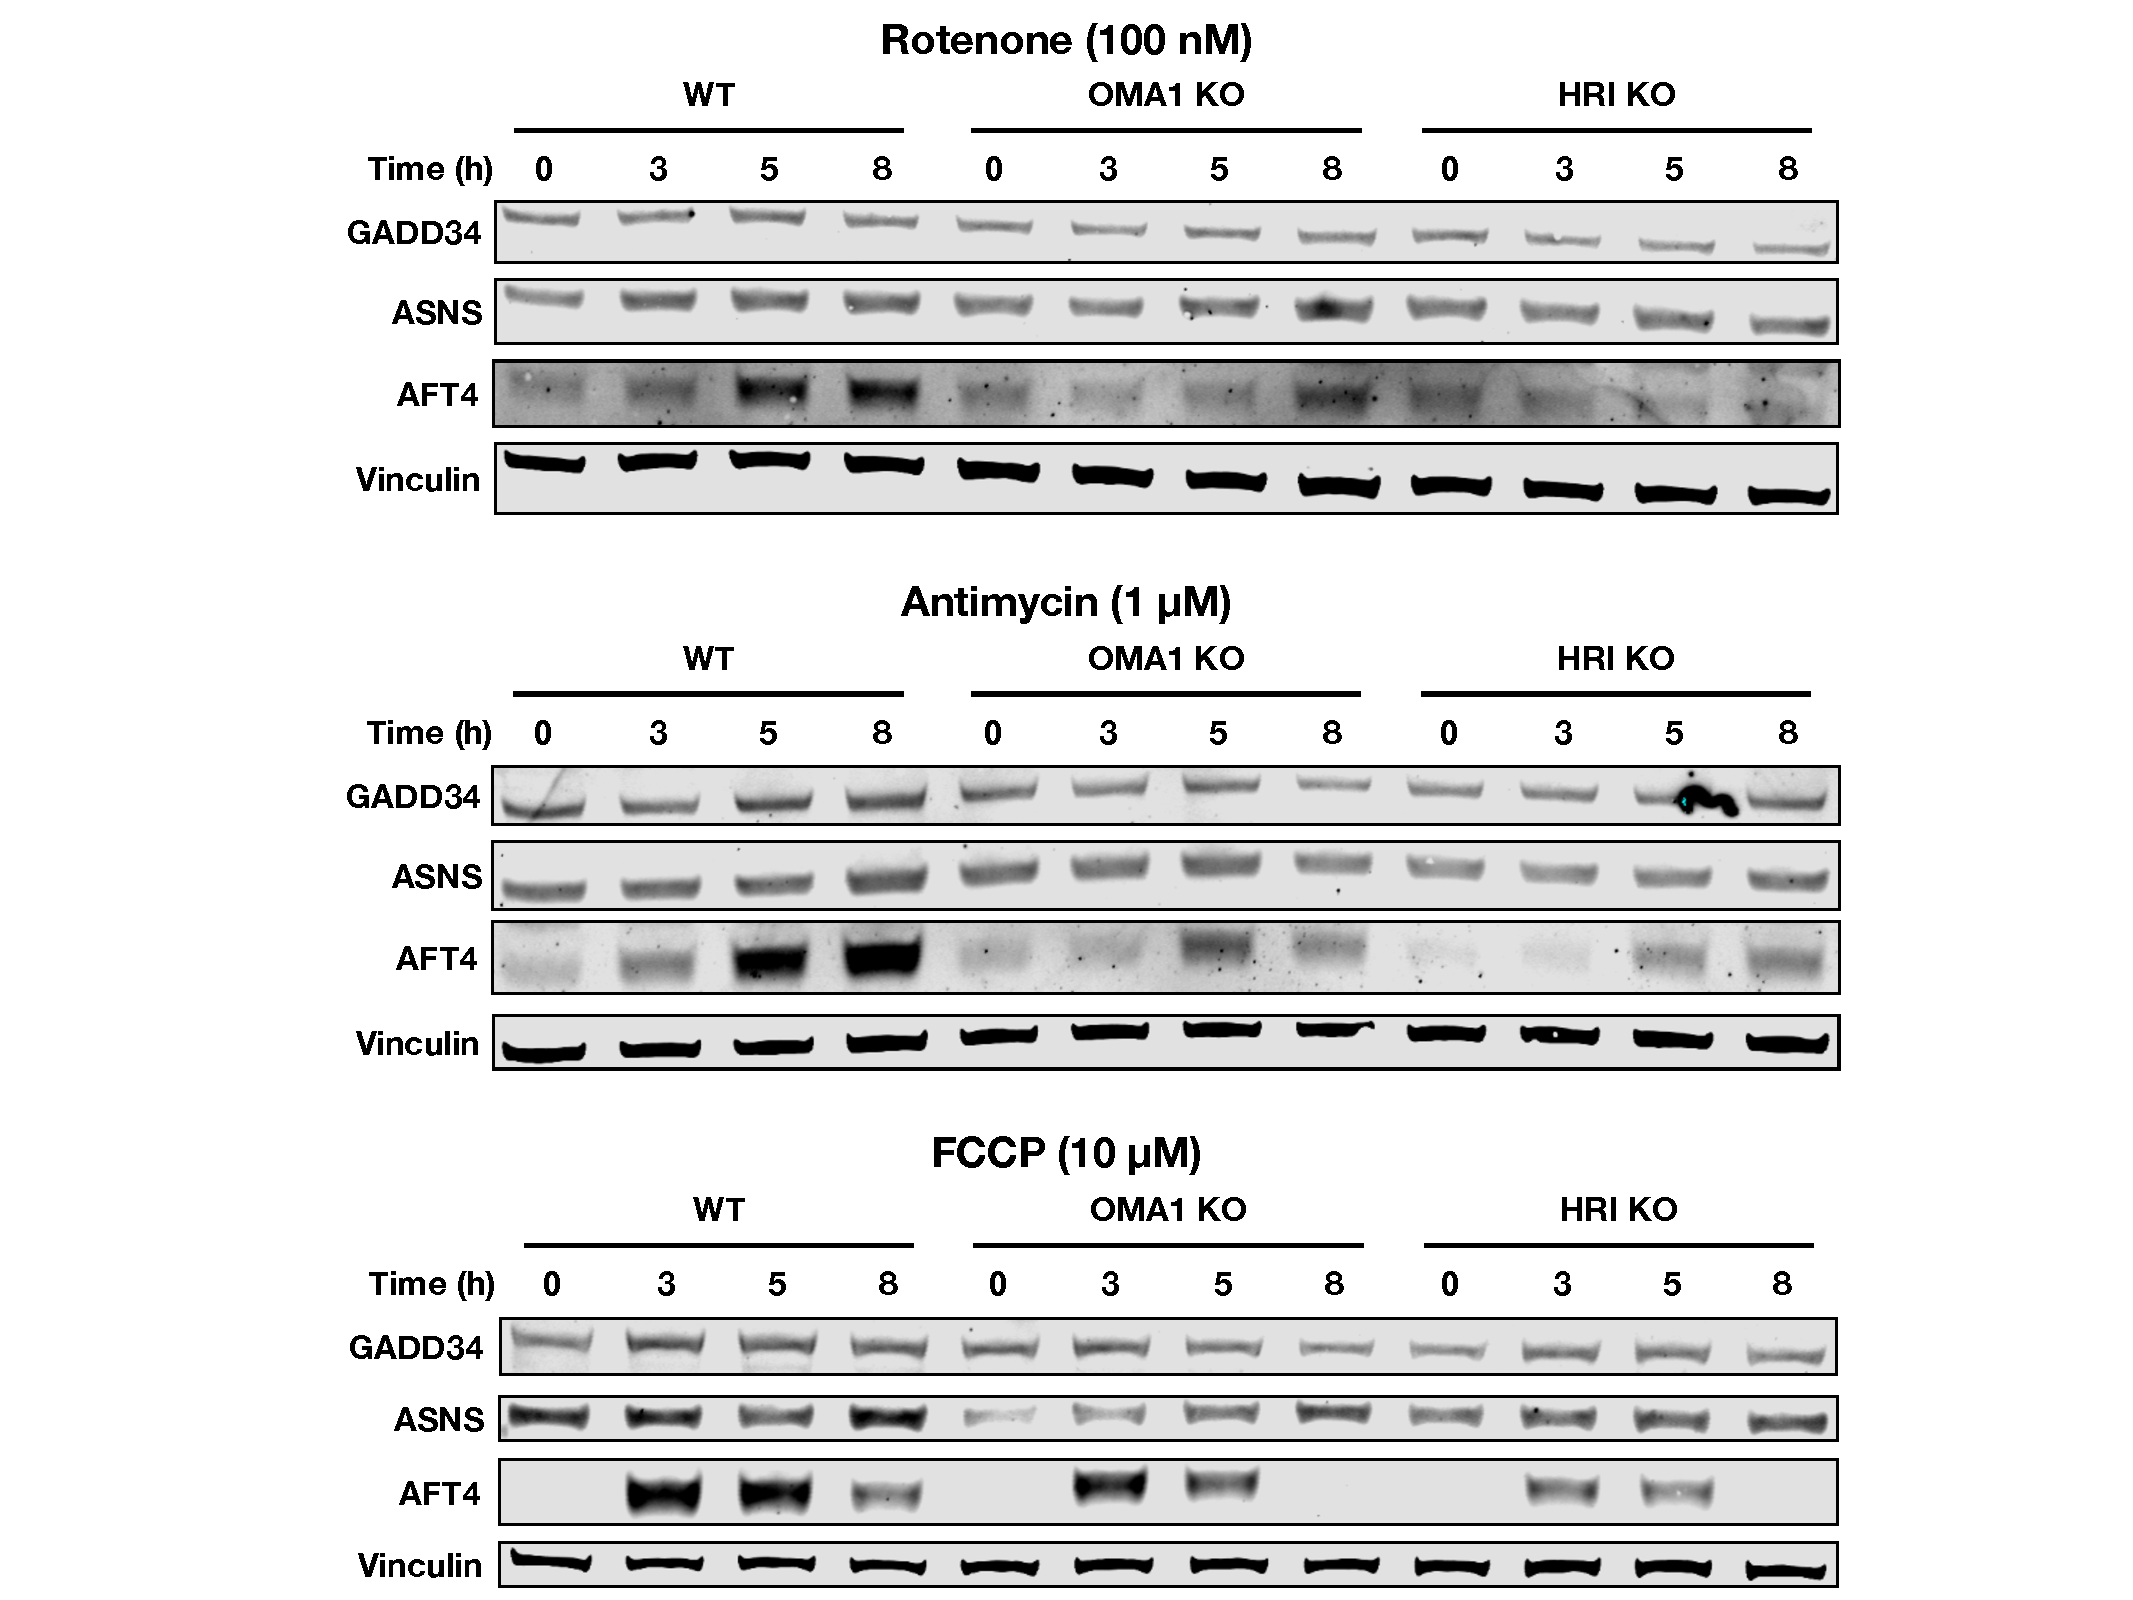
\includegraphics[width=0.65\textwidth]{figures/sapp/ISR/ATF4wes_OMA1_HRIpool.pdf}
    \caption[ATF4 post mito inhib. OMA1/HRI KO, western]{
    Same pooled knockout cells and handling as in figure \ref{fig:sapp:ISR:ATF4rep_OMA1_HRIpool}.
    Drugs spiked-in as 10x.
    }
    \label{fig:sapp:ISR:ATF4wes_OMA1_HRIpool}
\end{figure}






\subsection{OMA1/HRI relation to asp depletion induced ISR}
OMA1/HRI in HT1080 GOT DKO cells


\begin{figure}
    \centering
    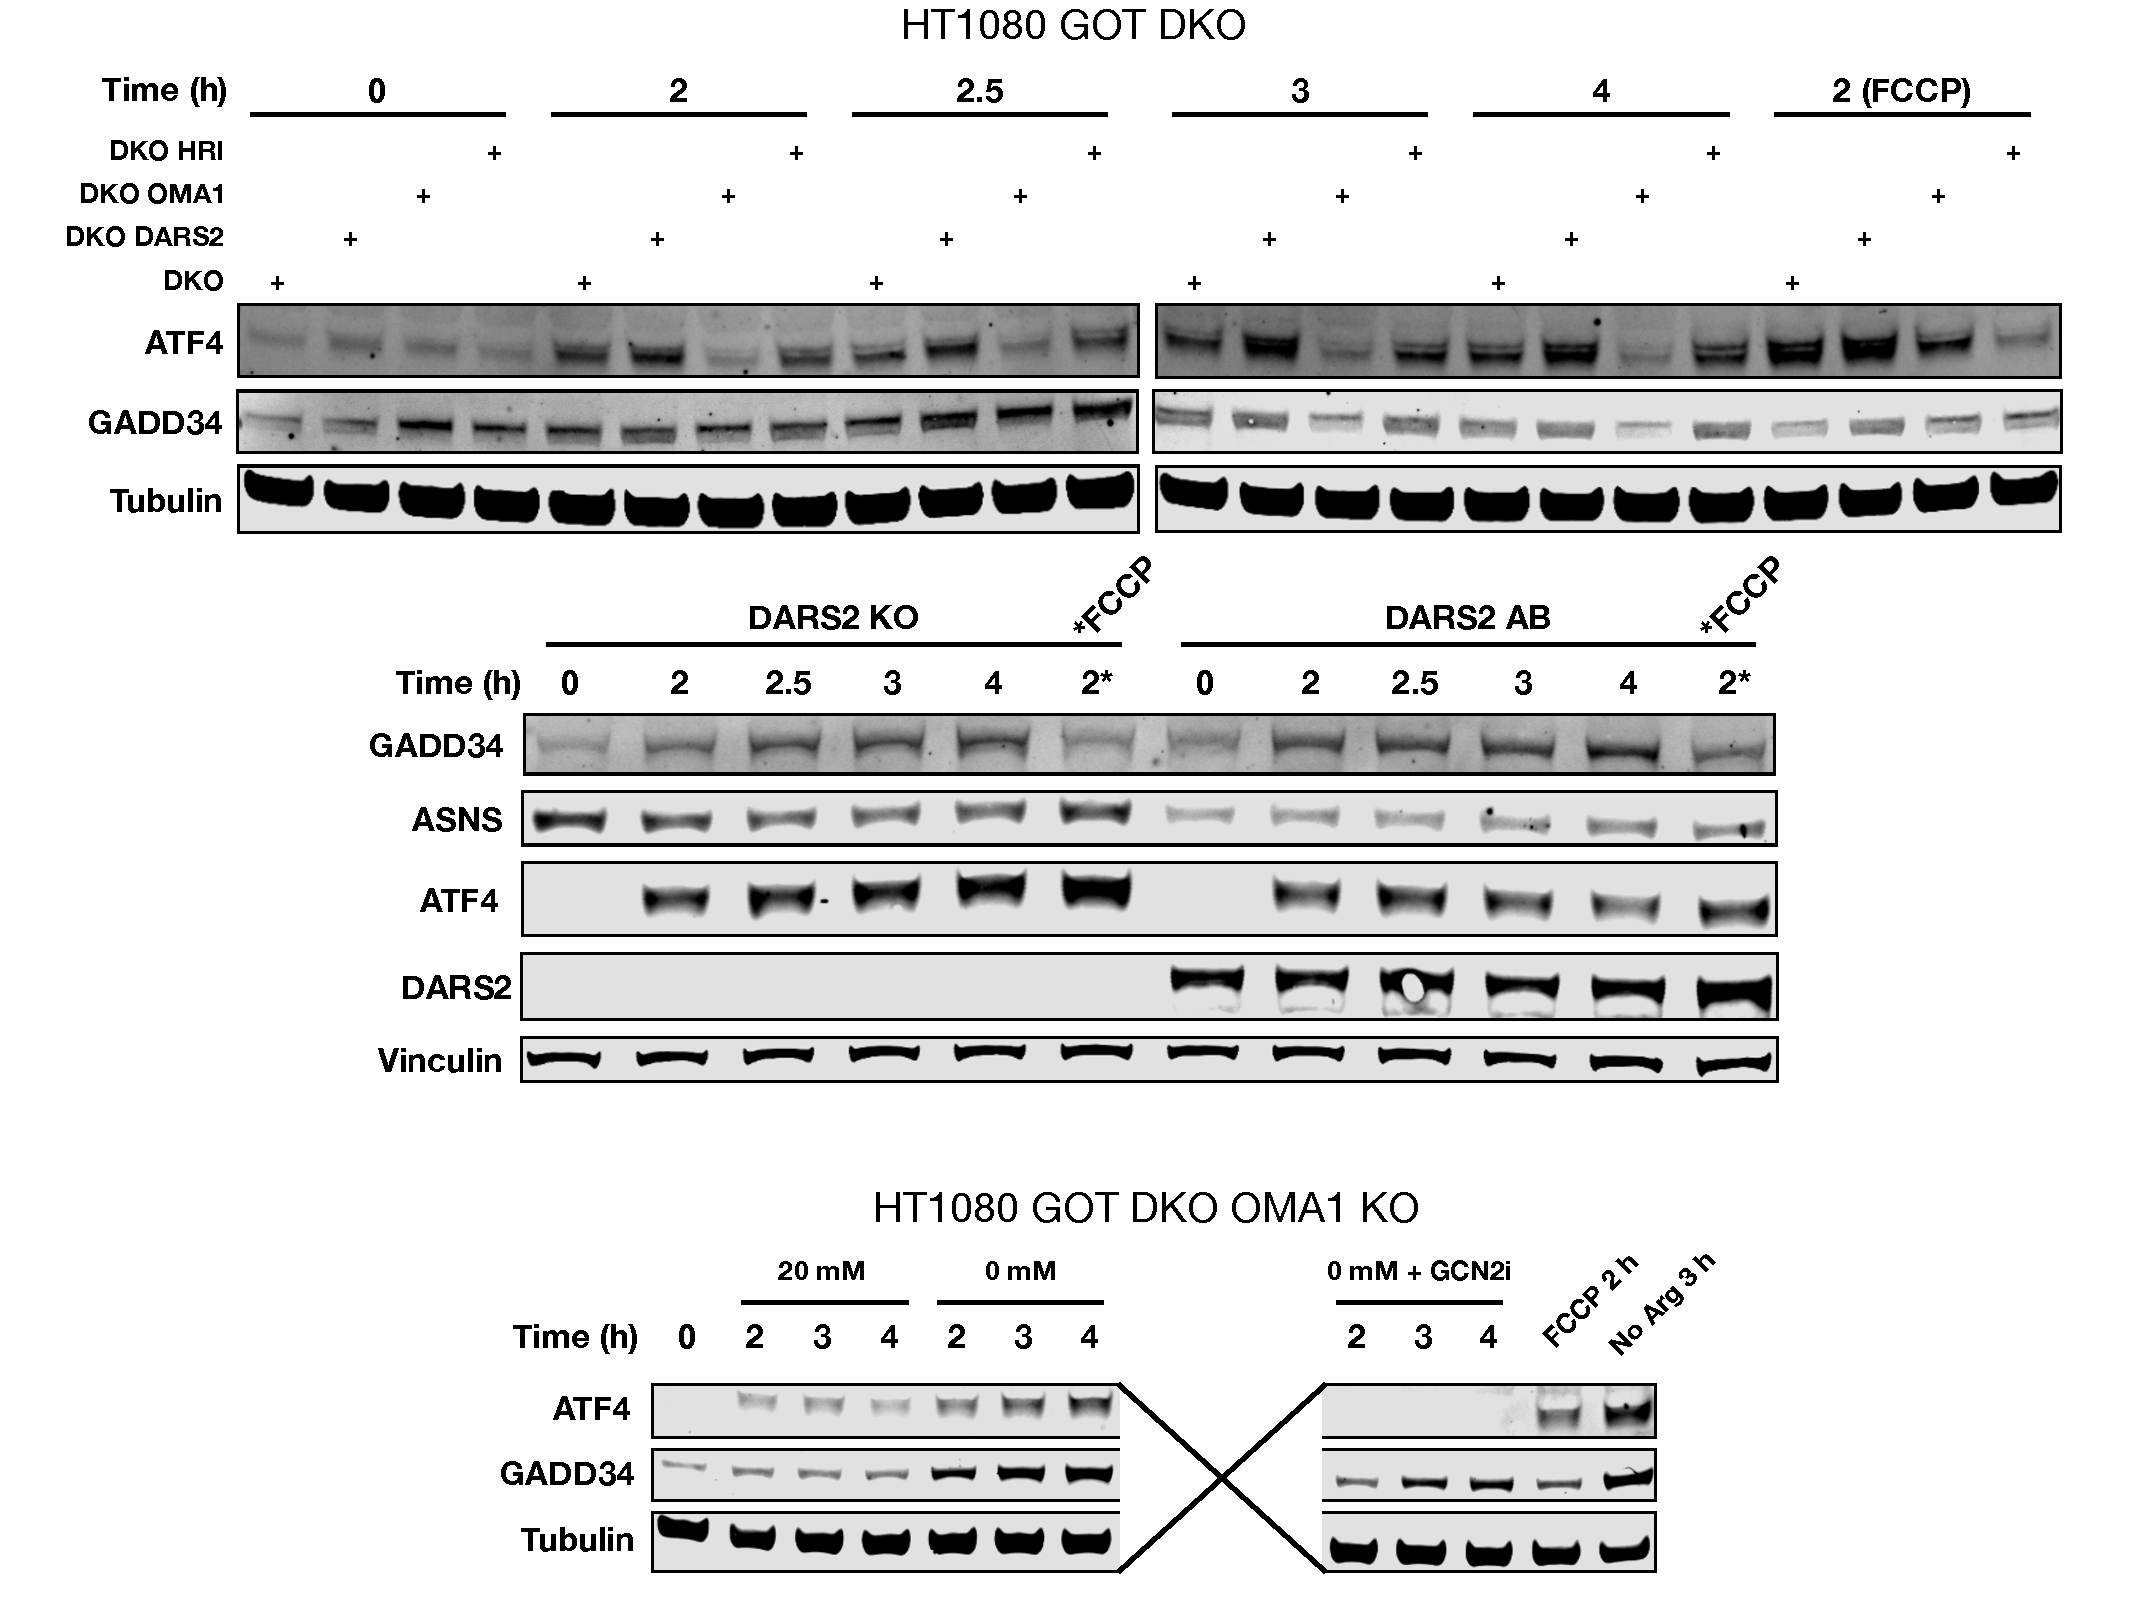
\includegraphics[width=0.95\textwidth]{figures/sapp/ISR/HT1080_DKO_KO_ISR.pdf}
    \caption[ATF4 post Asp depl. OMA1/HRI KO, western]{
    Effect of OMA1, HRI or DARS2 KO on aspartate induced ISR.
    Single cell clones validated for OMA1 and DARS2, only functionally validated for HRI, see figure \ref{fig:sapp:ISR:OMA1_HRI_DARS2_val}.
    }
    \label{fig:sapp:ISR:HT1080_DKO_KO_ISR}
\end{figure}

\begin{figure}
     \centering
     \begin{subfigure}[b]{0.49\textwidth}
         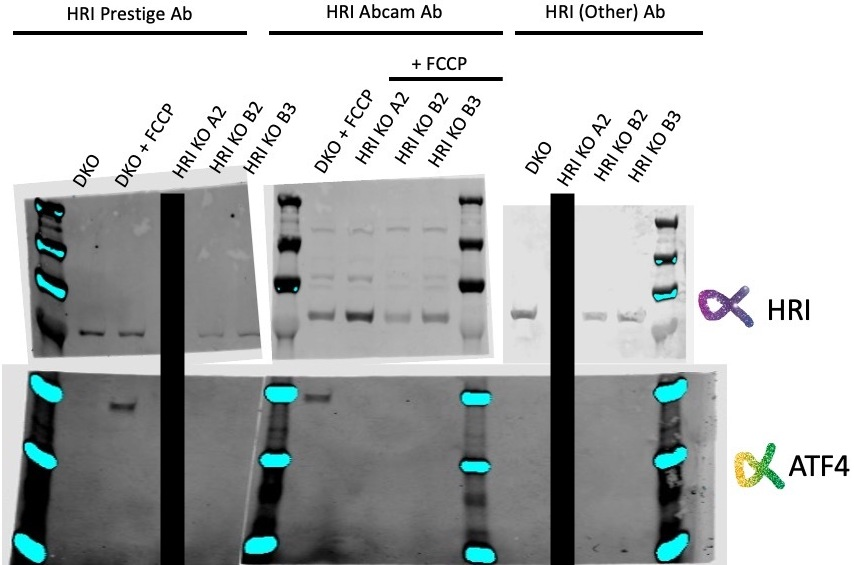
\includegraphics[width=\textwidth]{figures/sapp/ISR/HT1080_GOT_DKO_HRI_KO.jpeg}
         \caption{HT1080 GOT DKO, HRI KO western}
         \label{fig:sapp:ISR:HT1080_GOT_DKO_HRI_KO}
     \end{subfigure}
     \hfill
     \begin{subfigure}[b]{0.49\textwidth}
         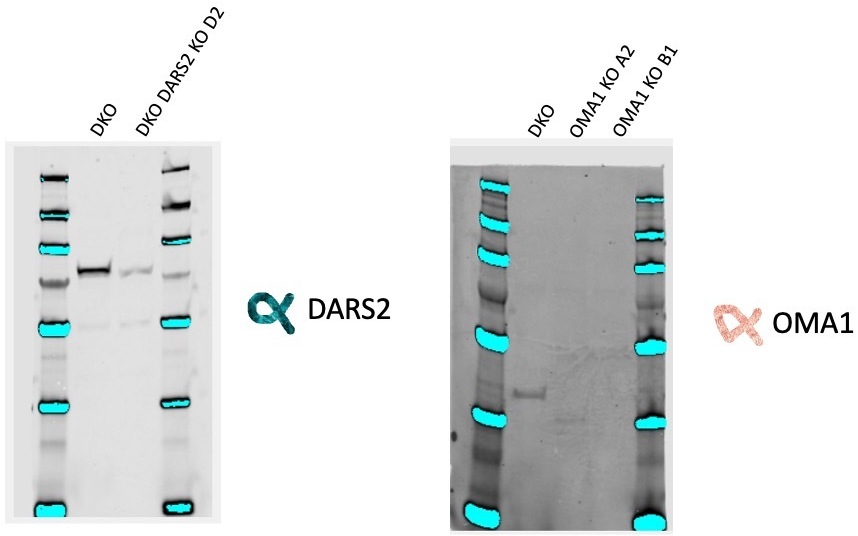
\includegraphics[width=\textwidth]{figures/sapp/ISR/HT1080_GOT_DKO_OMA1_DARS2_KO.jpeg}
         \caption{HT1080 GOT DKO, OMA1/DARS2 KO western}
         \label{fig:sapp:ISR:HT1080_GOT_DKO_OMA1_DARS2_KO}
     \end{subfigure}
     \hfill
        \caption[HT1080 GOT DKO, OMA1/HRI/DARS2 KO validation]{
        Western blot validations of OMA1, HRI and DARS2 knockouts.
        Image art credit: Ian Engstrom.
        }
        \label{fig:sapp:ISR:OMA1_HRI_DARS2_val}
\end{figure}









\subsection{GCN2 relation to rotenone induced ISR in 293T}
One would think that ETC inhibitor induced ISR is induced through Asp/Asn depletion and thus mediated by GCN2...
\begin{figure}
    \centering
    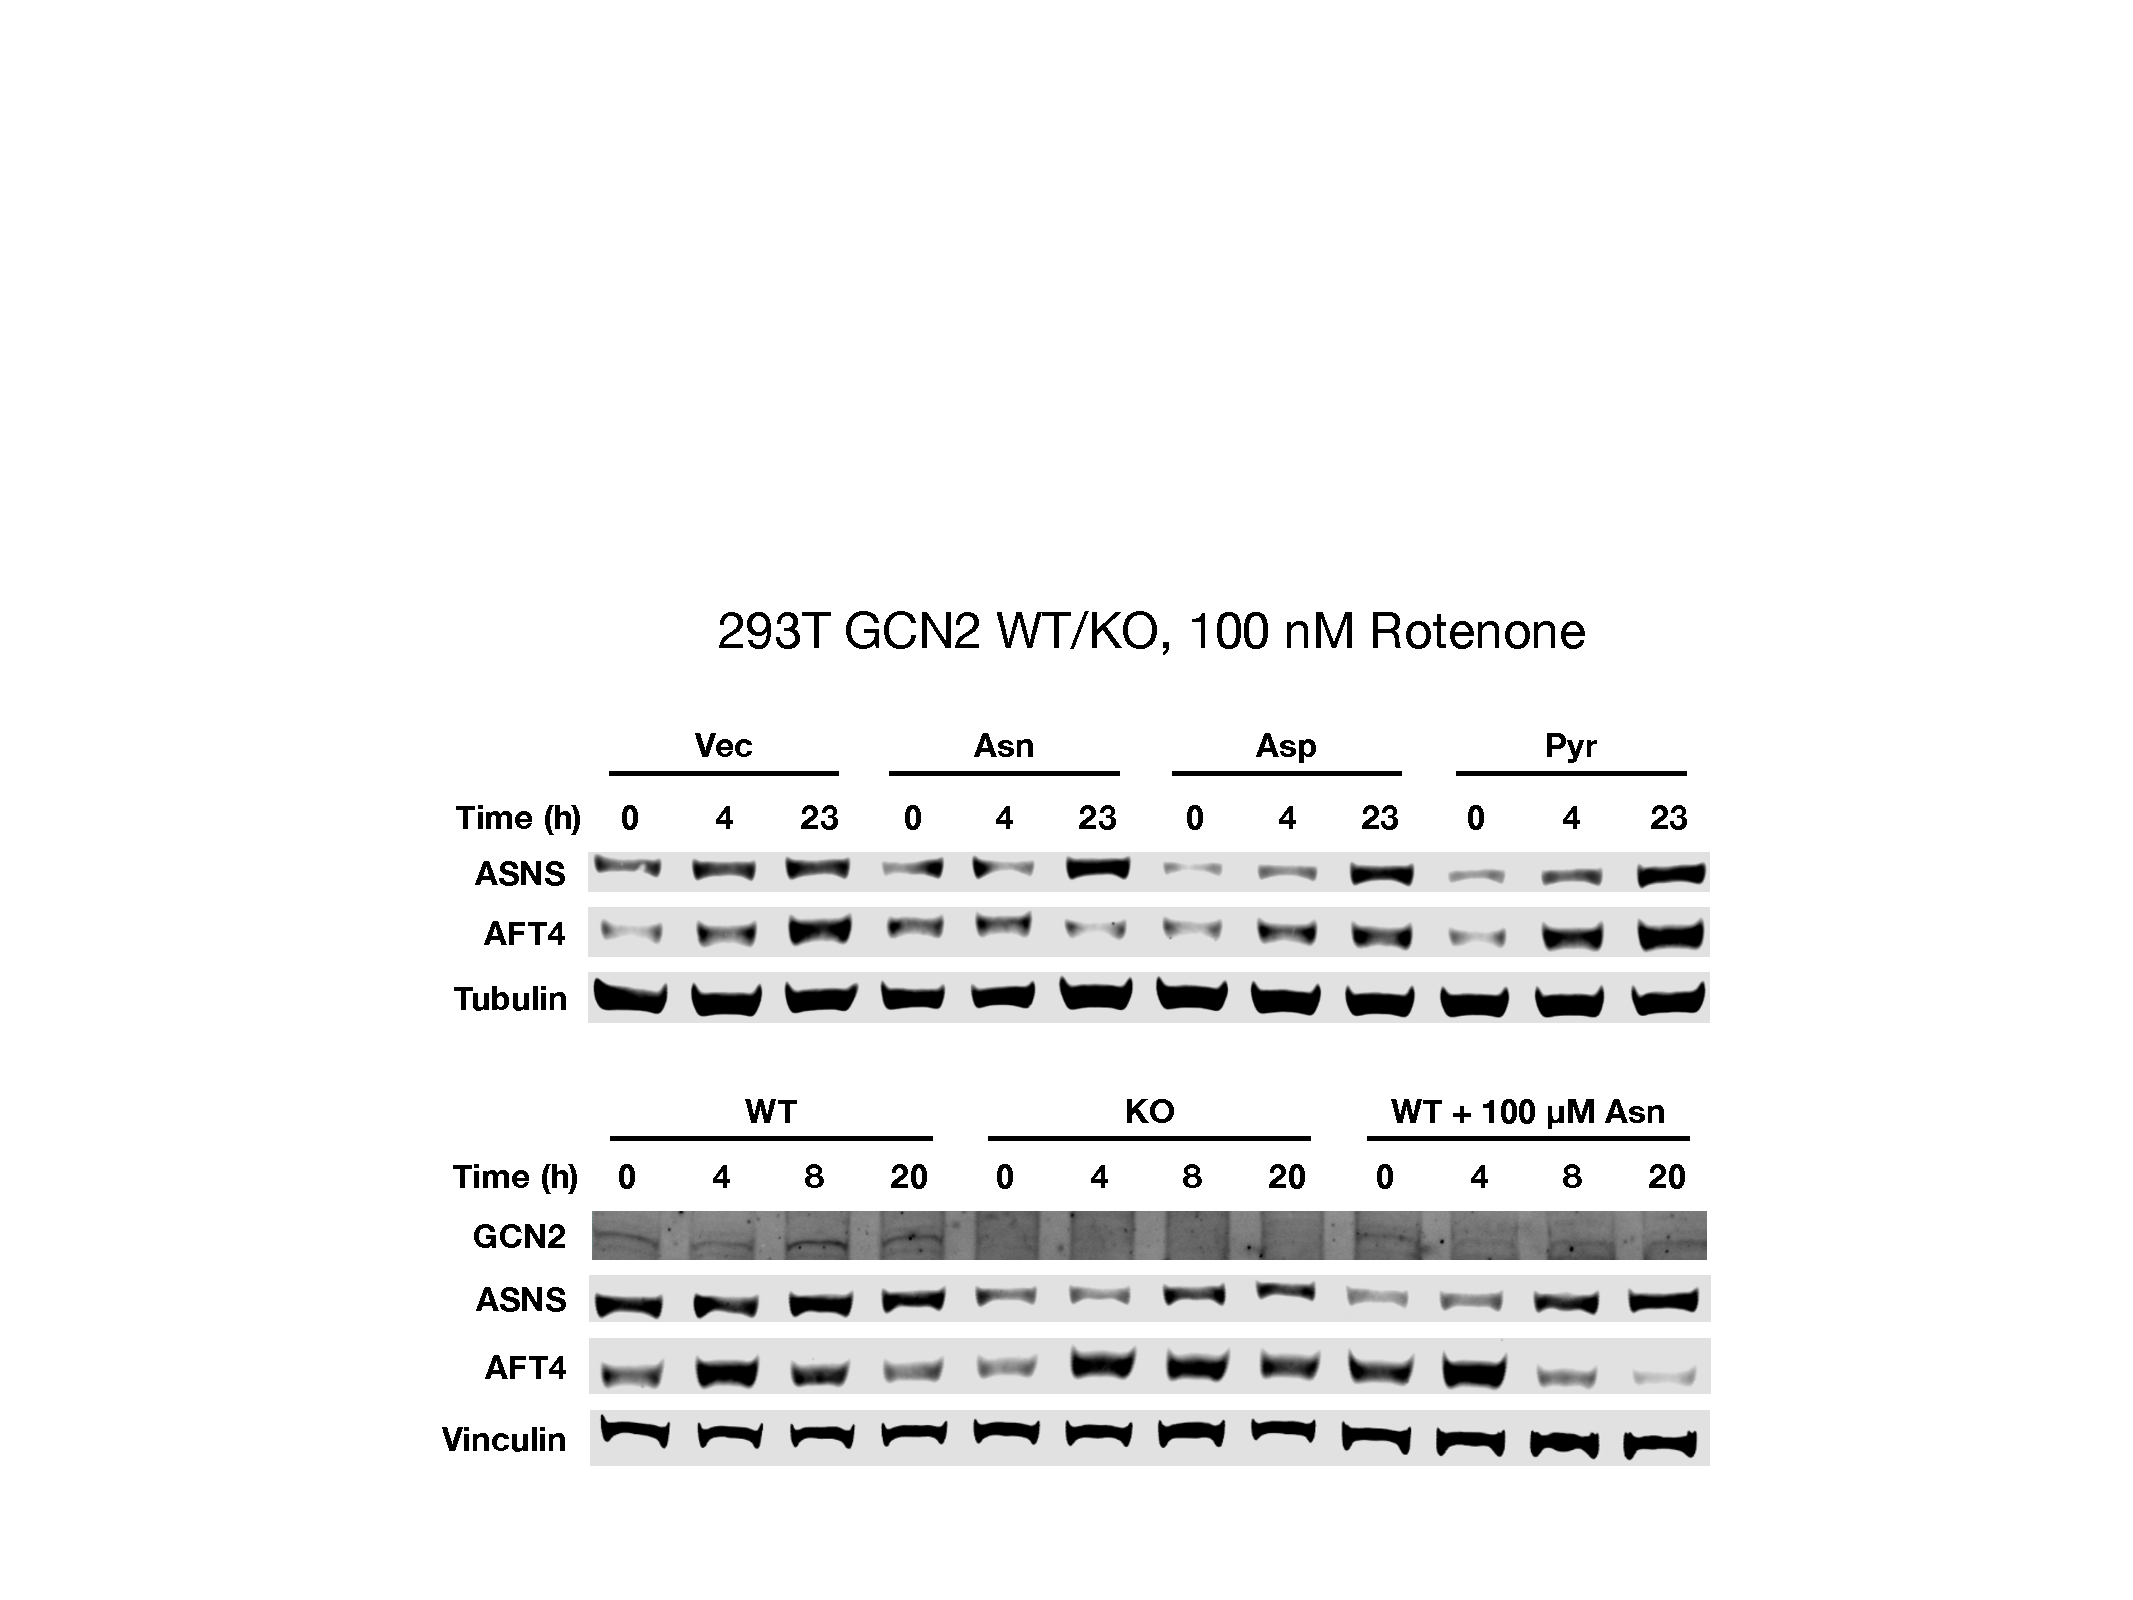
\includegraphics[width=0.70\textwidth]{figures/sapp/ISR/293T_GCN2_ISR.pdf}
    \caption[ATF4 post mito inhib. GCN2 KO, western]{
    Rotenone treatment was initiated by adding fresh media with 100 nM rotenone at time zero.
    Rescue conditions: Asn (500 µM), Asp (30 mM) or Pyr (2 mM) was also added to media >1 h before time zero.
    }
    \label{fig:sapp:ISR:293T_GCN2_ISR}
\end{figure}











\subsection{ASNS over-expression to ablate rotenone/antimycin induced ISR}


\begin{figure}
     \centering
     \begin{subfigure}[b]{0.49\textwidth}
         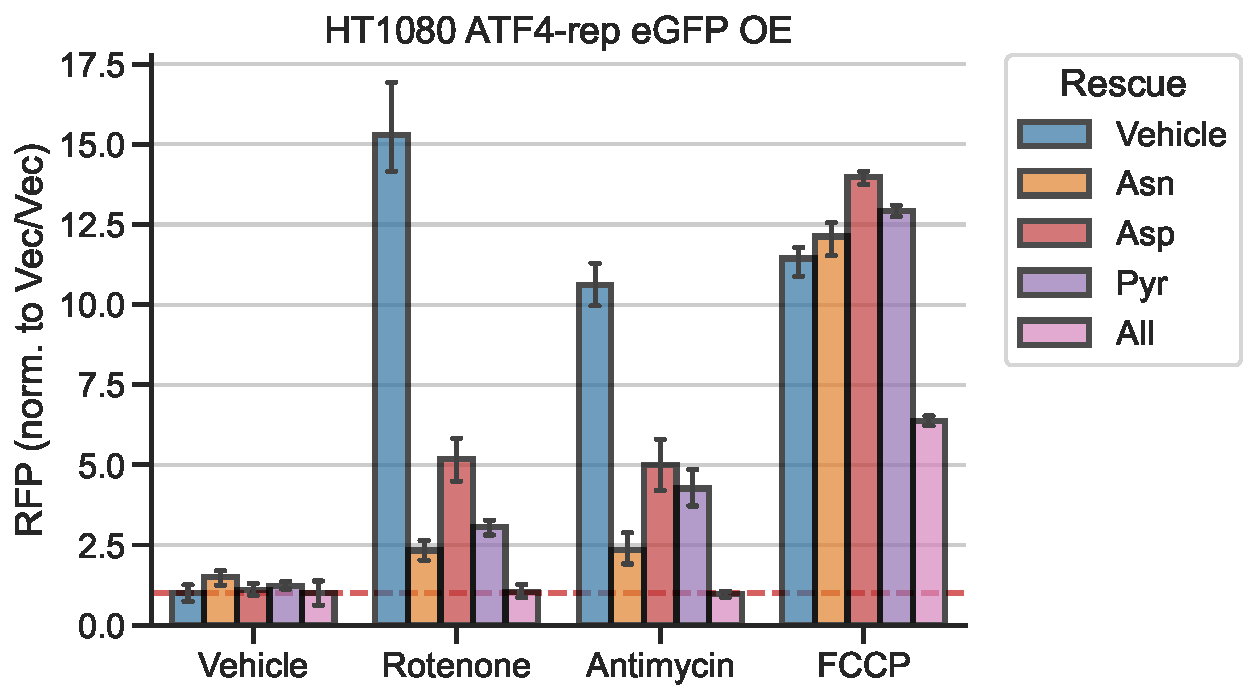
\includegraphics[width=\textwidth]{figures/sapp/ISR/HT1080_ATF4rep_eGFP_OE.pdf}
         \caption{ATF4 reporter, eGFP polyclonal}
         \label{fig:sapp:ISR:HT1080_ATF4rep_eGFP_OE}
     \end{subfigure}
     \hfill
     \begin{subfigure}[b]{0.49\textwidth}
         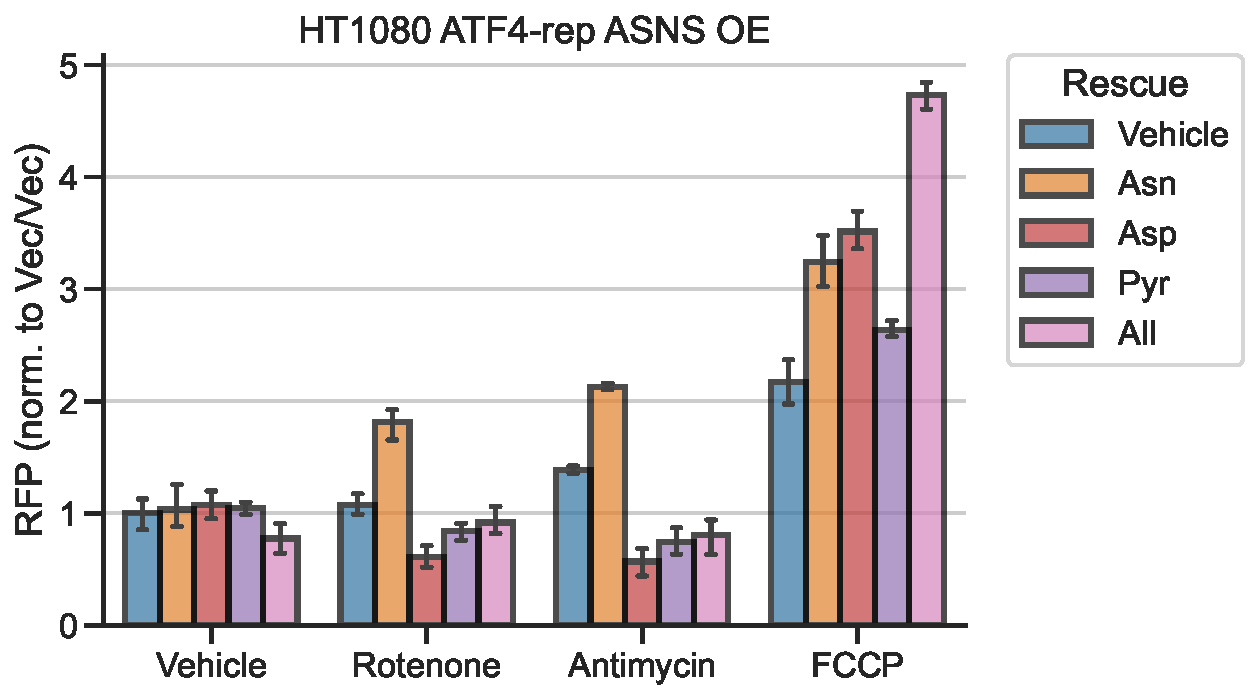
\includegraphics[width=\textwidth]{figures/sapp/ISR/HT1080_ATF4rep_ASNS_OE.pdf}
         \caption{ATF4 reporter, ASNS polyclonal}
         \label{fig:sapp:ISR:HT1080_ATF4rep_ASNS_OE}
     \end{subfigure}
     \hfill
     \begin{subfigure}[b]{0.6\textwidth}
         \centering
         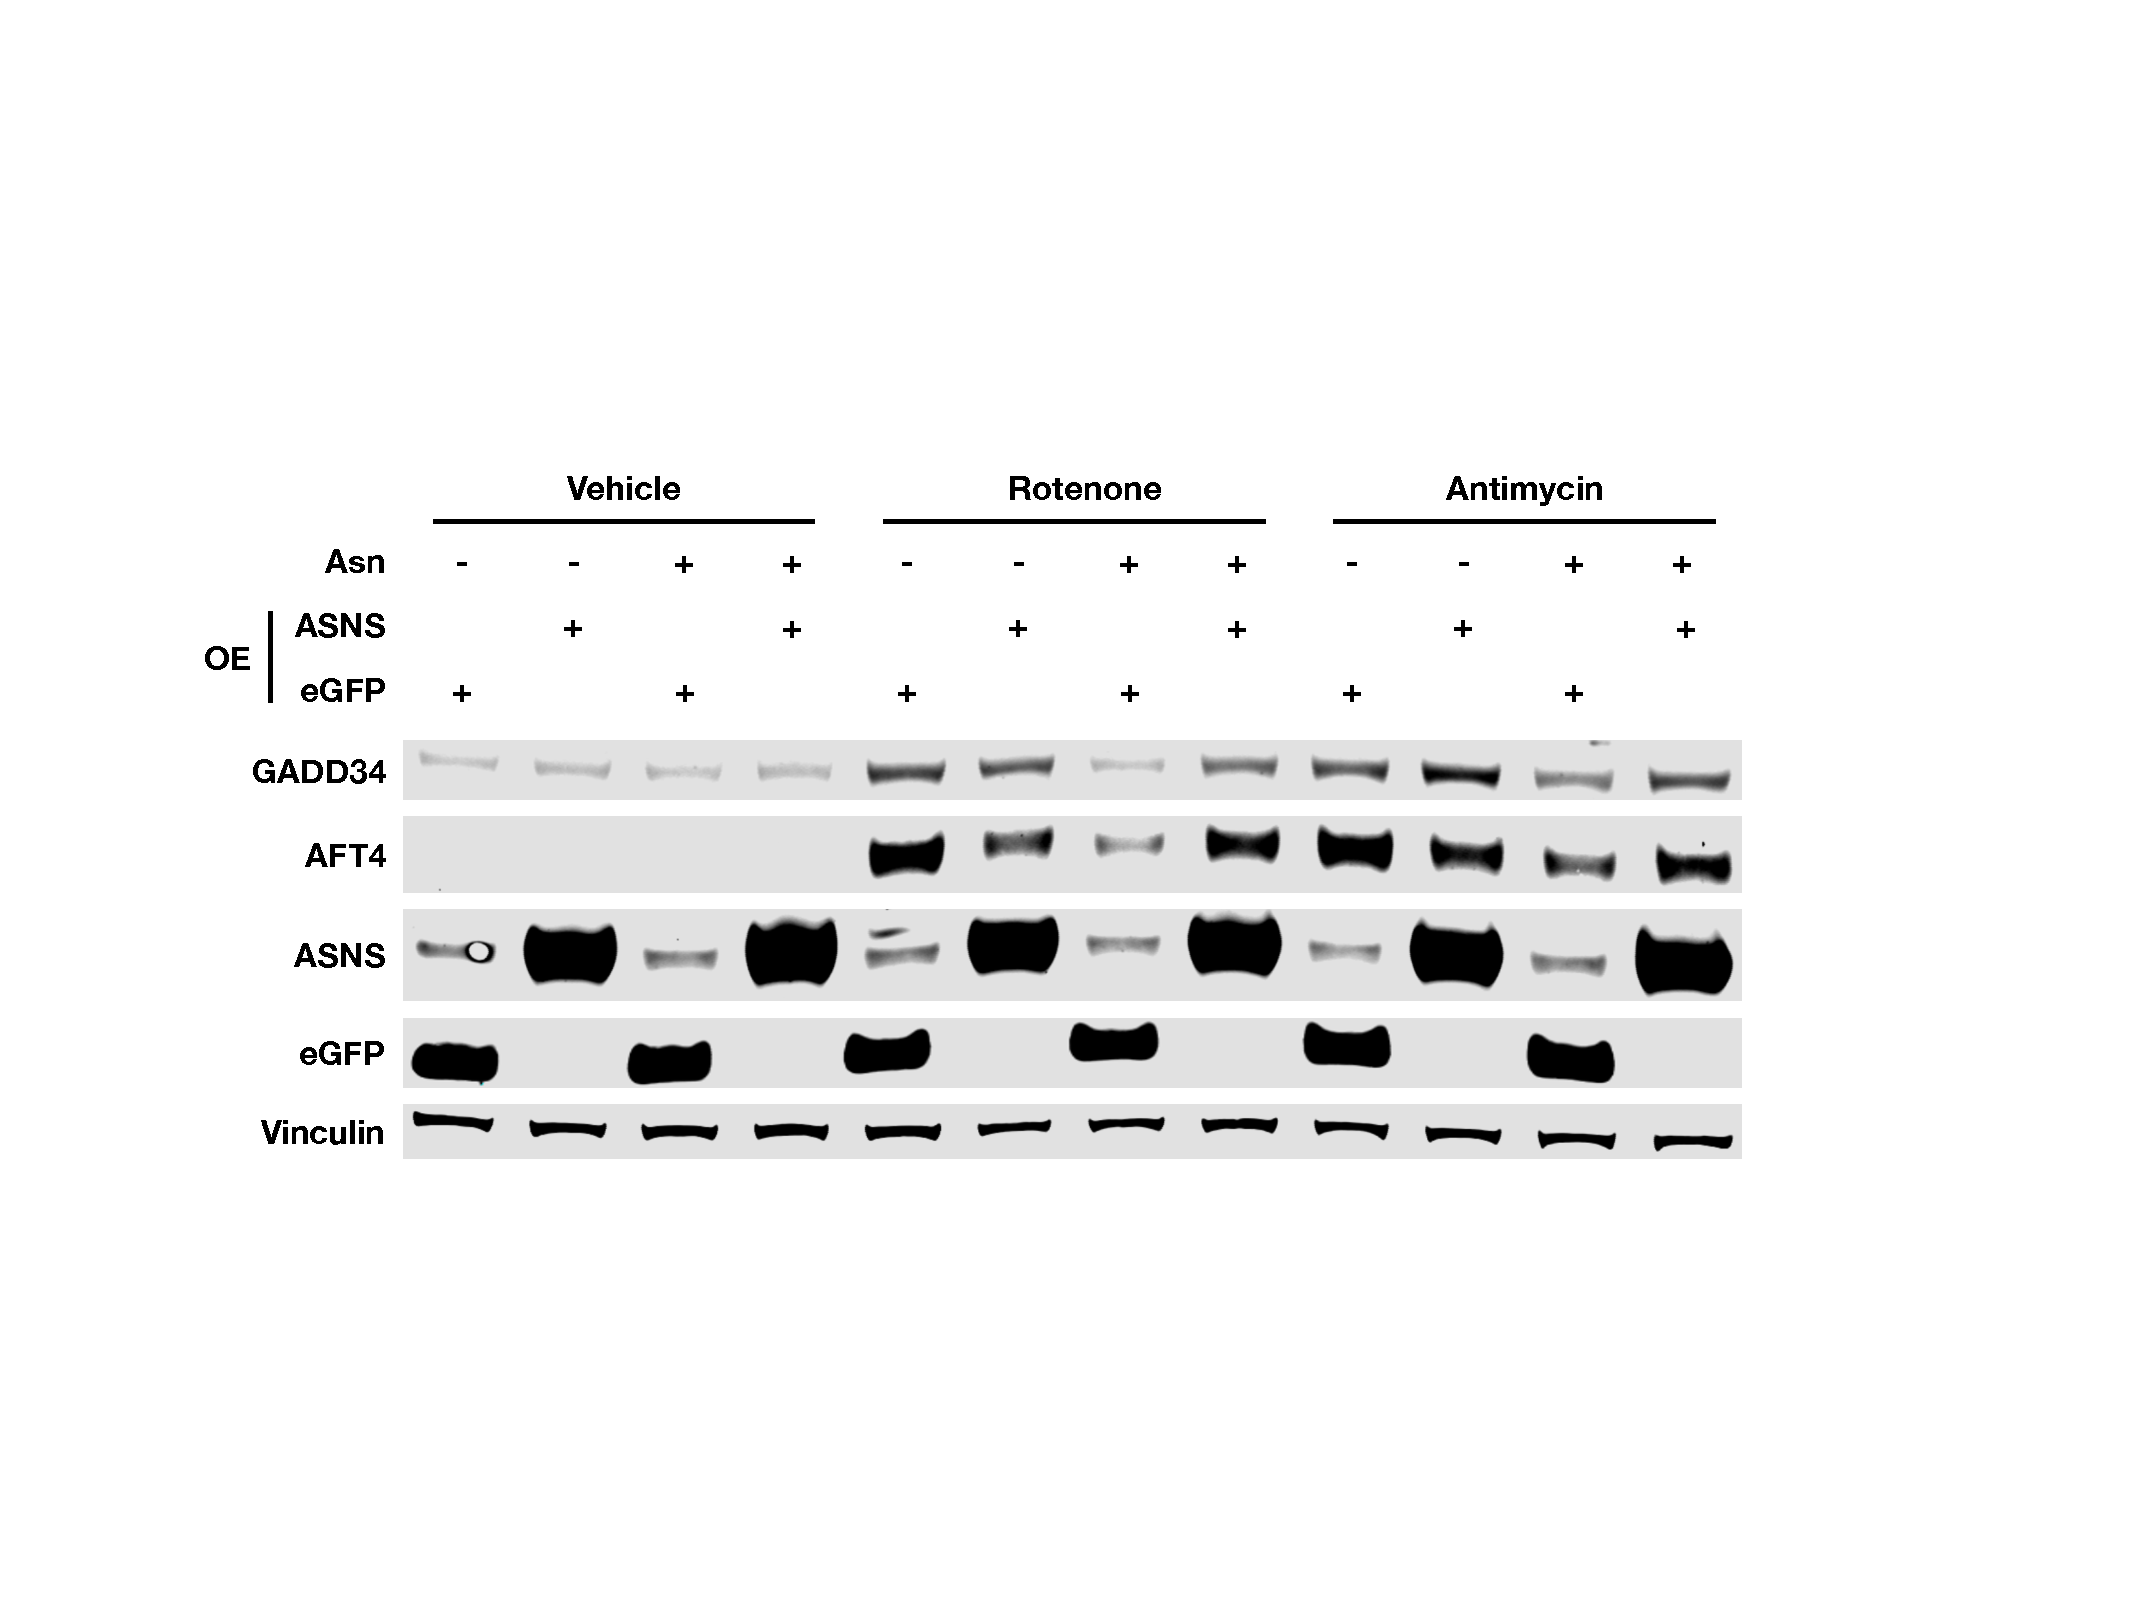
\includegraphics[width=\textwidth]{figures/sapp/ISR/HT1080_ISR_ASNS_OE.pdf}
         \caption{Western blot, eGFP/ASNS polyclonal}
         \label{fig:sapp:ISR:HT1080_ISR_ASNS_OE}
     \end{subfigure}
        \caption[ASNS, rotenone/antimycin induced ISR]{
        Effect of ASNS over-expression (eGFP control) on ATF4 reporter assay of ETC inhibitor induced ISR (parental HT1080 low baseline clone).
        }
        \label{fig:sapp:ISR:ASNS_ISR}
\end{figure}





